\documentclass{sigchi-ext}
% Please be sure that you have the dependencies (i.e., additional
% LaTeX packages) to compile this example.
\usepackage[T1]{fontenc}
\usepackage{textcomp}
\usepackage[scaled=.92]{helvet} % for proper fonts
\usepackage{graphicx} % for EPS use the graphics package instead
\usepackage{balance}  % for useful for balancing the last columns
\usepackage{booktabs} % for pretty table rules
\usepackage{ccicons}  % for Creative Commons citation icons
\usepackage{ragged2e} % for tighter hyphenation
\usepackage{float}
\usepackage{pgfgantt}
\usepackage{pgfgantt-custom}
\usepackage{verbatim}
\usepackage{gensymb} % for ohm-symbol

\usepackage{todonotes}

% For gifs?
%\usepackage{animate}

% \usepackage{marginnote} \usepackage[shortlabels]{enumitem}
% \usepackage{paralist}

%% EXAMPLE BEGIN -- HOW TO OVERRIDE THE DEFAULT COPYRIGHT STRIP --
 \copyrightinfo{Permission to make digital or hard copies of all or
 part of this work for personal or classroom use is granted without
 fee provided that copies are not made or distributed for profit or
 commercial advantage and that copies bear this notice and the full
 citation on the first page. Copyrights for components of this work
 owned by others than ACM must be honored. Abstracting with credit is
 permitted. To copy otherwise, or republish, to post on servers or to
 redistribute to lists, requires prior specific permission and/or a
 fee. Request permissions from permissions@acm.org.\\
 {\emph{CHI'17}}, May 16--May 22, 2017, Copenhagen, Denmark. \\
 Copyright \copyright~2017 ACM ISBN/17/05...\$15.00. \\
 DOI string from ACM form confirmation}
%% EXAMPLE END

\title{GUARDIAN SUIT: Baby monitoring onesie using eTextile}

\numberofauthors{3}
% Notice how author names are alternately typesetted to appear ordered
% in 2-column format; i.e., the first 4 authors on the first column and
% the other 4 authors on the second column. Actually, it's up to you to
% strictly adhere to this author notation.
\author{%
  \alignauthor{%
    \textbf{Madrigal N. Totayo}\\
    \affaddr{University of Copenhagen} \\
    \affaddr{Universitetsparken 5} \\
    \affaddr{2100 Copenhagen} \\
    \affaddr{vnw888@alumni.ku.dk} } \vfil \alignauthor{%
    \textbf{Mark Wulff}\\
    \affaddr{University of Copenhagen}\\
    \affaddr{Universitetsparken 5}\\
    \affaddr{2100 Copenhagen} \\
    \email{lrh211@alumni.ku.dk} }  \vfil \alignauthor{%
    \textbf{Mark J. Jacobi}\\
    \affaddr{University of Copenhagen}\\
    \affaddr{Universitetsparken 5}\\
    \affaddr{2100 Copenhagen} \\
    \email{dcz738@alumni.ku.dk} } }

% Paper metadata (use plain text, for PDF inclusion and later
% re-using, if desired)
\def\plaintitle{SIGCHI Extended Abstracts Sample File: Note Initial
  Caps} \def\plainauthor{First Author, Second Author, Third Author,
  Fourth Author, Fifth Author, Sixth Author}
\def\plainkeywords{SIDS; eTextile; monitoring; breathing; lying position.}
\def\plaingeneralterms{Documentation, Standardization}

%% Set up our PDF with metadata
\hypersetup{%
  pdftitle={\plaintitle}, pdfauthor={\plainauthor},
  pdfkeywords={\plainkeywords}, }

% \reversemarginpar%

\begin{document}

\maketitle

% Uncomment to disable hyphenation (not recommended)
% https://twitter.com/anjirokhan/status/546046683331973120
\RaggedRight{}

% Do not change the page size or page settings.
\begin{abstract}
  The most important rule of Abstracts is that they describe the work, not the paper. Include, at most, one sentence of motivation. Save the rest of your motivation for the Introduction. Effective Abstracts focus on two things: (1) Describing what was done. (2) Describing what was found (key results). Be specific about your key findings. Instead of "many" say "84\%". Keep the Abstract to one paragraph and fewer than 200 words.
\end{abstract}

\keywords{\plainkeywords}

\category{J.3}{Health and Medical systems}{Medical information systems}
% See http://www.acm.org/about/class/ccs98-html for all (men denne er den eneste som passer til os)

\section{Introduction}
Parents and guardians of infants are often worried about their health. Because of this, various baby monitoring technologies have been developed. These monitoring devices checks the sleeping environment for the baby (e.g. critical shifts in the temperature of the room) and alarms the parent or guardian. A majority of these products have an object present near the infant's crib, which we find to be rather clunky and can be misleading (i.e. false positives). Unfortunately, they do not give any information of which position the baby is lying in and whether it is breathing or not.

%\begin{comment}
\marginpar{%
  \vspace{-10pt} \fbox{%
    \begin{minipage}{0.925\marginparwidth}
    \textbf{Guardian Suit} \\
      \begin{figure} [H]
    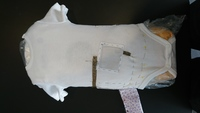
\includegraphics[width=1.0\textwidth]{img/resize/w200/prototype_overview}
    \caption{Guardian Suit (onesie - no breath sensor as we need it seperately to test it)}
\end{figure}
      \begin{figure} [H]
    \includegraphics[width=1.0\textwidth]{img/resize/w200/breath_sensor}
    \caption{The breath sensor, mounted on a strip of cotton fabric for testing}
\end{figure}
    \end{minipage}}\label{sec:sidebar} }
%\end{comment}

Many recommendations for the infants sleeping positions and environments has been made in order to lower the probability of Sudden Infant Death Syndrome (SIDS)\footnote{\url{https://en.wikipedia.org/wiki/Sudden_infant_death_syndrome}}. After years of research by the American Academy of Pediatrics (AAP) \cite{aap-1992,aap-1996,aap-2005} the main recommendations for minimizing the probability of SIDS is to detect:
\begin{itemize}
  \item Whether the infant is breathing or not.
  \item When the infant changes position.
\end{itemize}
To address these points we developed Guardian Suit, a onesie with one-dimensional textile sensors sewn into it as such: (1) around the chest area, (2) on the lower-back, (3) stomach, and (4) one on each side.

The first sensor introduced (1) consists of a piezoresistive elastic polymer
which decrease in resistance when stretched. This allows for detecting whether
the infant is breathing or not.\\
The sensors for the sides, stomach and back (2,3,4) consists of a piece of
piezoresistive fabric in-between two pieces of conductive fabrics. 
They decrease in resistance when pressure is applied to them. 
These sensors are placed as such, in order to detect whether the infant is in a
prone (i.e. on the stomach), supine (i.e. on the back) or lateral (i.e. on the
side) position.


% Ville skulle forklare noget om isolering af de ledende stoffer, men vi kan også bare fjerne det
\begin{comment}
Furthermore, as our product is electrical, we don't want the possibility of
hurting the baby e.g. by getting electrocuted. For this, we created strips out
of conductive fabric that were sewn into the onesie. 
These are then connected to the development board by crimping the
sensors\footnote{\url{https://www.pololu.com/product/1928\#lightbox-picture0J3280;main-pictures}} or by using
snaps\footnote{\url{https://www.sparkfun.com/products/11347}}.
\end{comment}

To test this crude first generation prototype, we manufactured a doll which 
mimic some properties of a baby, e.g. weight and shape. We put the Guardian Suit
on the doll and moved it into various positions. We found that the pressure pads
worked very well in detecting the positioning of the doll. As for the breathing
sensor, we tested it on ourselves as we did not have access to a baby. Though
it were able to detect breathing, the very subtle stretch in the piezoresistive
elastic polymer is hard to detect and body movement would overshadow any output
from breathing. However, it still was possible to produce a curve from which 
we are able to identify breaths.\todo{results?}

% Måske bare fjerne og så fortsætte?
\begin{comment}
In the following, we will describe our findings of how the infant should interact with the apparatus. Thus, we had to build it with the following in mind: (1) sensor construction and placement techniques, (2) connecting the sensors to the development board without the use of wires, and (3) usage scenarios and possible feedback from the readings.
\end{comment}


\section{Guardian Suit}
\colorbox{cyan}{Modified universal onesie bought from a generic baby clothing store}
\colorbox{cyan}{Argumantation for for why this is a
better approach: Affordable, non-intrusive?}
\colorbox{cyan}{Picture overview}
\colorbox{cyan}{key components}

\section{Motivational scenario}
The parents of an infant realizes that it is dozing off, and decides to put the infant in a crib for a nap, where the infant is dressed with the Guardian Suit beforehand. The infant is initially placed on its back in the crib, and the parents goes about with their work. Whenever the infant changes position, either to one of the sides or on the stomach, the parents are notified by the pressure pads embedded in the suit in order to take action. The same with the breathing sensor, when the infant isn't breathing \colorbox{cyan}{25-40} consecutive breaths per minute, the parents are notified, and thus, can take immediate action.

\section{Related work}
Many products has been developed to allow parents and guardians to monitor their infants. One of them is the Georgia Tech Wearable Motherboard (GTWM)\footnote{\url{http://www.gtwm.gatech.edu/}}. Initially developed in collaboration with the US Navy Department to monitor a soldier's vital signs by detecting the penetration of e.g. bullets and shrapnel, it was later augmented to monitor an infant's breathing or heart rate by using cardiorespiratory sensors on a vinyl strap, as described by Fantauzzacoffin et al. \cite{p285-fantauzzacoffin}. The engineers had created it by weaving signal transmission lines and integrated the sensors into a onesie. One mother didn't mind her infant to be surrounded by wires from the device, and found it to be quite comfortable.

Kroutil et al. \cite{a33-kroutil} used electrically conductive stranded yarn as sensors, placed underneath the lower bed sheet to detect respiration among individuals.

The sensors measured the respiratory activity by the alteration of electrical capacitance of the chest area. This was done so one could monitor patients respiration without inconveniencing them with wiring and sensors attached to their bodies.

Another bedsheet monitor was proposed by Huang et al. \cite{a18-huang}. Embedded with pressure sensors and in conjunction with collated data, they were able to detect whether the person was breathing or not within a certain time interval, corresponding to a predetermined minimum breathing rate.

Even though creating the sensors within the fabric of the surface the infant is lying on during sleep has produced satisfactory results \cite{a18-huang, a33-kroutil}, we have chosen another approach. Guardian Suit combines the wearability, comfort, and ease of use of GTWM\footnote{\url{http://www.gtwm.gatech.edu/}} \cite{p285-fantauzzacoffin} with the pressure sensing technologies used in the bedding solutions. We receive feedback whenever the infant is in either position i.e. prone (stomach), supine (back) or lateral (side). With the electrical elastic polymer described earlier we are able to detect the breathing rate of the baby. Finally, with constraints as proposed by Huang et al. \cite{a18-huang}, we can detect whenever any individual is in a critical state.

We are using piezoresistive conductive
stretchable fabric for breathing detection. However, an alternate solution method to the breathing sensor
could be investigated based on the research of Vogl et al. \cite{stretcheband}, who
test various stitching patterns of conductive thread and the resistance measured
when stretched.


\clearpage

\section{Technical evaluation of materials/sensors}

\subsection{EeonTex piezoresistive elastic polymer}

%\begin{comment}
\marginpar{%
  \vspace{-10pt} \fbox{%
    \begin{minipage}{0.925\marginparwidth}
    \textbf{Piezoresistive elastic polymer evaluation} \\
      \begin{figure} [H]
    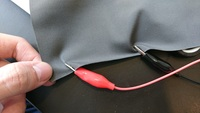
\includegraphics[width=1.0\textwidth]{img/resize/w200/breathing_sensor}
    \caption{Test of the piezoresistive elastic polymer using crocodile clip wires.}
\end{figure}
      \begin{figure} [H]
    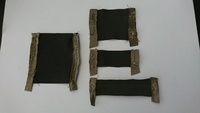
\includegraphics[width=1.0\textwidth]{img/resize/w200/stretch_sensors}
    \caption{The different sizes of stretch sensors we tested (missing 1.0x5.0cm)}
\end{figure}
      \begin{figure} [H]
    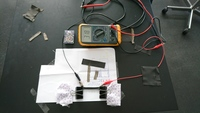
\includegraphics[width=1.0\textwidth]{img/resize/w200/stretch_test_setup}
    \caption{Test setup for the stretch sensors, results in table \ref{tab:stretch-test}}
\end{figure}
    \end{minipage}}\label{sec:sidebar} }
%\end{comment}

For the breathing sensor we will use the EeonTex piezoresistive elastic polymer.
This polymer has the property that the resistance is decreased when the fabric
is stretched.

From the consultation of some eTextile experts, we determined
that tuning the sensor will be a three step approach.\\
First, we will find the piece size of the material which
is the most sensitive given the limited size we need it to be
to fit on the chest. Next, we will experiment with various
resistors to find the best suitable one for our input range.
Thirdly, configure the smoothing software for the sensor readings.

As we need some indication of the amount the material will
be stretched, we measured the circumference of the chest
when fully exhaled, fully inhaled and a regular breath
(this will vary depending on person).
\begin{table}[H]
  \centering
  \begin{tabular}{l r}
    % \toprule
    & \multicolumn{1}{l}{\small{\textbf{Breath circumference measure}}} \\
    \cmidrule(r){1-2}
    {\small\textit{State}}
    & {\small \textit{circumference (cm)}} \\
    \midrule
    Full exhale    & 101.0 \\
    Full inhale    & 107.0 \\
    Regular exhale & 104.2 \\
    Regular inhale & 105.5  \\
    % \bottomrule
  \end{tabular}
  \caption{Measurements of chest circumference when breathing. Used for testing the Eeontex material.}~\label{tab:circumference}
\end{table}
From the above table we get an idea of how much a single breath affects the circumference
in an adult male. Though this is not representative of a baby, due to the
inaccessibility of one and that we want to develop a first iteration prototype, this
will be our basis of the breathing sensor.

We see that the difference in a full forced inhale/exhale is around 6 cm. whereas regular
breathing only results in around 1 cm in difference.\\
We have experimented with the different sizes of the Eeontex conductive piezoresistive
stretch fabric. From the breath circumference table we can see the change varies in cm and construct a simple experiment in order to evaluate the change in resistance given
different fabric sizes, as noted in the table below.
\begin{table}[H]
  \centering
  \begin{tabular}{l r r r r}
    % \toprule
    & \multicolumn{4}{l}{\small{\textbf{Stretch sensor test results}}} \\
    \cmidrule(r){2-4}
    {\small\textit{Size (cm x cm)}}
    & {\small \textit{+0.0cm}}
    & {\small \textit{+0.5cm}}
    & {\small \textit{+1.0cm}}
    & {\small \textit{+1.5cm}} \\
    \midrule
    1.0x5.0    & 306-307 & 241-242 & 217-218 & 202-203\\
    2.5x5.0    & 101-102 & 78-77 & 63-64 & 58-59 \\
    2.5x7.5    & 122-123 & 108-109 & 89-90 & 83-84 \\
    5.0x5.0    & 63-64 & 53-54 & 39-40 & 37-38 \\
    5.0x7.5    & 44-45 & 47-48 & 39-40 & 35-36 \\
    % \bottomrule
  \end{tabular}
  \caption{Resistance measured using volt-meter in k$\ohm$}~\label{tab:stretch-test}
\end{table}
We performed the test with two sets of the material sizes.
We discovered during the first test that if the material
is stretched beyond a certain limit, the material gets
damaged such the piezoresistive property changes. In our case,
we found that it becomes less sensitive.

From the test, we have determined the 2.5x5.0cm size
performed the best and therefore we will proceed with this
configuration.

\clearpage

\subsection{Pressure sensors}
The position sensors will be eTextile pressure sensors by putting two conductive
fabrics with a piezoresistive fabric in-between which changes resistance when
pressed.

For testing
the efficiency of the sensor, we started by making a
simple prototype before the actual sensors.
We used some copper wires as connectors, 1.4 mm, after verifying the pad with
crocodile clip wires. When we tested the pad, the idle resistance measured when on the table was
around 900 (due to fabric deformities this would vary). by slight touch, the resistance dropped to around 400. From this observation we determined that 
this type of pad would suffice as pressure sensor.

%\begin{comment}
\marginpar{%
  \vspace{-160pt} \fbox{%
    \begin{minipage}{0.925\marginparwidth}
    \textbf{Pressure sensor evaluation} \\
      \begin{figure} [H]
   \centering 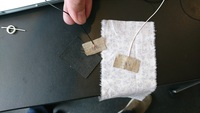
\includegraphics[width=0.85\textwidth]{img/resize/w200/pressure_sensor.jpg}
    \caption{The prototyping of the eTextile pressure sensor pad.}
\end{figure}
      \begin{figure} [H]
   \centering 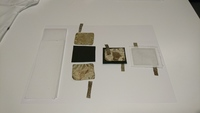
\includegraphics[width=0.85\textwidth]{img/resize/w200/pressure_sensor2.JPG}
    \caption{Overview of the final pressure sensor pad construction (materials and assembly).}
\end{figure}
      \begin{figure} [H]
   \centering 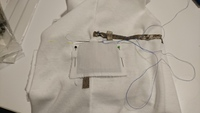
\includegraphics[width=0.85\textwidth]{img/resize/w200/pe_integration.JPG}
    \caption{Pressure sensor sewn into Guardian Suit.}
\end{figure}
    \end{minipage}}\label{sec:sidebar3} }
%\end{comment}

Construction of the sensors embedded into Guardian Suit, we used 
silver plated nylon and conductive thread (coated with micron-thick layer of 
natural silver). As we want to demonstrate that all materials used can be
composed of eTextiles, we chose this over copper wiring.

When constructing the pads, all the conductive fabrics (non stretch) were
burned around the edges to keep the fabric from fraying.
For wrapping and keeping in place, we used a thin cotton
fabric which is non-conductive and kept together using
fabric glue.
For connectors we use the silver plated nylon fabric to make a stripe around
the stomach area for the ground connector \todo{5v istedet antager jeg? (Mark J.)} which all pads will be connected to.

For the wiring of each of the analog input to each pad, we used conductive
thread. In our prototype the thread leads out of the onesie by a line of
fabric to make it less restrictive when manipulating the doll which it is
put on. However, as future work the microcontroller would be embedded into
the onesie as well and use wireless connectivity to transmit data.

To evaluate the pads which will be embedded into Guardian Suit, we applied 
increasing weights and measured the resistance using a volt meter.\\
As we did not have weights we used danish coins, 20 and 5 kr. coins, which both
weigh (sampled using 5 coins) 9.3g each. Therefore we can treat each of them as
being the same weight.
\begin{figure} [H]
   \centering 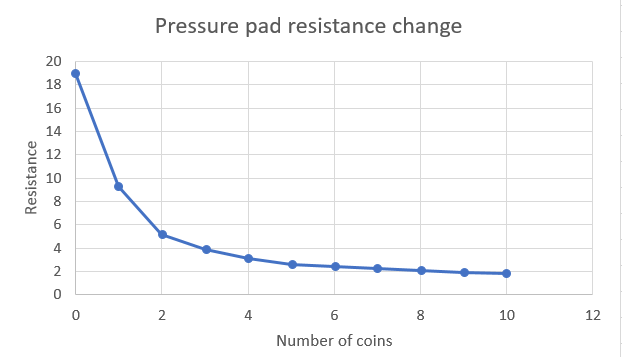
\includegraphics[width=0.45\textwidth]{img/chart.PNG}
    \caption{Resistance change by weight (m$\ohm$)}
\end{figure}
From the chart we can see that around 100g of force will drop the resistance
by around 90\%. From these results we determined that the sensors would be suitable
as a newborn weighs on average 3.5kg.

\clearpage

\section{Prototype construction (Mark + Mark)}
What separates Guardian Suit from conventional alternative baby monitors 
(e.g. cameras and noise sensors) is its relative low cost and monitors the
baby directly and not the environment around it. The 
sensors are not difficult to produce and can be integrated into any fabric-based
onesie by sewing. The only significant component in Guardian Suit is the
micro-controller which would be embedded into the onesie also.\\
To construct the prototype we made the sensors and evaluated them as
described in the precious sections. Then we bought a cotton leg and arm-less
onesie from H\&M and embedded our sensors into it.

For connectors, we used silver plated nylon and conductive thread (coated with
micron-thick layer of natural silver. We also evaluated these against copper
wiring in the pressure sensor evaluation section. The issue with these
connectors is that because they are plated with silver, washing prototype
would over time reduce the conductivity of the material.

\colorbox{cyan}{A little about how our Arduino-setup works with plots (Mark J.)}.
\colorbox{cyan}{like... en 2-3 paragrapher)}.


\section{Prototype evaluation (ALL on Tuesday)}
\colorbox{cyan}{breathing sensor on mark}.\\
\colorbox{cyan}{move doll around}.

\section{Future work (All on tuesday - Mark W. udkast)}
We used piezoresistive elastic polymer for our breathing sensor. Using this,
we were able to detect breathing but with very limited signal. Also, muscle flex
would produce much more prominent signals. We don't expect this to be any
different given any other materials or stretch sensors. However,
based on the research of Vogl et al. \cite{stretcheband} it would be interesting
to see what signal is produced when making the same kind of stitch pattern on
the test area and evaluate the signal output.

The Guardian Suit works in theory by the test on the doll in the study. However,
the prototype has yet to be evaluated on an actual baby which would provide the
most accurate real world usage as the product is intended for babies. However,
another place to start would be to build it into an adult size piece of clothing
and try it on an adult.

Generally, the prototype can be further developed in multiple ways. Most imediately would be to 
find a micro-controller to be embedded into the onesie. Also, given the connectors currently are just
sewn into the onesie, finding a way to insulate them would be something to consider in a future
iteration of the prototype.

\section{Conclusion (All on tuesday)}
\colorbox{cyan}{The paper is concluded}.




\balance{}

\bibliographystyle{SIGCHI-Reference-Format}
\bibliography{sample}

\end{document}

%%% Local Variables:
%%% mode: latex
%%% TeX-master: t
%%% End:
